\documentclass[11pt]{article}
\usepackage{mystyle}

\title{Structure Tensor Analysis Update}
\author{Scott Trinkle}
\date{April 9, 2018}

\begin{document}

\maketitle

The concept of structure tensor analysis seems to have been initially developed
in a 1987 computer vision paper by Bigun and Granlund~\cite{Bigun1987}. It has
since been used for a variety of computer vision and materials science
applications, including finding the orientation of textile fibers with
synchrotron microCT imaging~\cite{Straumit2015}. It was notably applied to
validating diffusion MRI with 2D histology by Budde~\cite{Budde2012,Budde2013}
and others. Schilling~\cite{Schilling2016,Schilling2018} and
Khan~\cite{Khan2015} have extended the analysis to 3D for the same purpose. In
this report, I am following the derivation and notation given in Appendix A of
the most recent Schilling paper~\cite{Schilling2018}.

\section{Derivation}

Consider a three-dimensional intensity image, $f(x,y,z)$, with gradient:
\begin{equation}
  \label{eq:grad}
  \nabla f_{\sigma_d} = {\left(f_x, f_y, f_z\right)}^T
\end{equation}
which is calculated using Gaussian derivative filters:
\begin{align}
  \label{eq:gradcomps}
  f_x = g_{x,\sigma_d} \ast f & &  f_y = g_{y,\sigma_d} \ast f & &  f_z = g_{z,\sigma_d} \ast f
\end{align}
where $\ast$ denotes the convolution operator and $g_{i, \sigma_d}$ denotes the
spatial derivative in the $i$-direction of a 3D~Gaussian, $g_{\sigma_d}$, with
standard deviation $\sigma_d$:
\begin{equation}
  \label{eq:gauss}
  g_{\sigma_d}(x,y,z) = \frac{1}{\left(2\pi\sigma_d^2\right)^{3/2}}\text{ exp}\left\{-\frac{x^2 + y^2 + z^2}{2\sigma_d^2}\right\}
\end{equation}

The image gradient is used to construct a ``gradient square tensor'' by taking
the dyadic product of the gradient vector with itself:
\begin{equation}
  \label{eq:GST}
  \text{GST}(x, y, z)_{\sigma_d} = \nabla f_{\sigma_d} \nabla f_{\sigma_d}^T =
  \begin{pmatrix}
    f_x^2 & f_x f_y & f_x f_z \\
    f_x f_y & f_y^2 & f_y f_z \\
    f_x f_z & f_y f_z & f_z^2 \\
  \end{pmatrix}
\end{equation}

Each element of the GST is then averaged over a local neighborhood to create the
voxel-wise structure tensor. Most groups have performed averaging using a 3D
Gaussian filter with standard deviation $\sigma_N$:
\begin{equation}
  \label{eq:ST}
  \text{ST}_{\sigma_N}\left(\nabla f_{\sigma_d}\right) = g_{\sigma_N} \ast
  \left(\nabla f_{\sigma_d} \nabla f_{\sigma_d}^T \right) = g_{\sigma_N} \ast
  \begin{pmatrix}
    f_x^2 & f_x f_y & f_x f_z \\
    f_x f_y & f_y^2 & f_y f_z \\
    f_x f_z & f_y f_z & f_z^2 \\
  \end{pmatrix}
\end{equation}

This results in a 3$\times$3 symmetric, positive semi-definite, rank-two tensor
at every voxel. The direction of minimal intensity variation is given by the
eigenvector of this tensor corresponding to the smallest eigenvalue. We make the
assumption that this direction also describes the corresponding fiber
orientation of that voxel.

The eigenvalues can be used to estimate the certainty in the estimated fiber
orientation, i.e., the voxel-wise ``anisotropy index,'' which I will refer to as
AI. Several specific metrics have been proposed:

The textile group~\cite{Straumit2015} uses the ratio of minimum and maximum
eigenvalues:
\begin{equation}
  \label{eq:eigratio}
  \text{AI} =
  \begin{cases}
    1 - \frac{\lambda_3}{\lambda_1} & \lambda_1 > 0\\
    0 & \lambda_1 = 0
  \end{cases}
\end{equation}
where $\lambda_1$, $\lambda_2$ and $\lambda_3$ are the primary, secondary and
tertiary eigenvalues of the structure tensor.

Schilling~\cite{Schilling2016, Schilling2018} uses the ``Westin-measure'':
\begin{equation}
  \label{eq:westin}
  \text{AI} = \frac{\lambda_2 - \lambda_3}{\lambda_1}
\end{equation}

Khan~\cite{Khan2015} uses ``fractional anisotropy,'' which is also used in DTI:
\begin{equation}
  \label{eq:FA}
  \text{AI} = \sqrt{\frac{1}{2}\frac{(\lambda_1-\lambda_2)^2 + (\lambda_2-\lambda_3)^2 +
      (\lambda_1 - \lambda_3)^2}{\lambda_1^2 + \lambda_2^2 + \lambda_3^2}}
\end{equation}

The AI is then commonly used to threshold the image $f$, so voxels with low
anisotropy are not included in the orientation distribution.

\section{Implementation}

\subsection{Gaussian filtering}

Currently, the Gaussian filtering is being implemented with the
\href{https://docs.scipy.org/doc/scipy-0.16.1/reference/generated/scipy.ndimage.filters.gaussian_filter.html}{ndimage.gaussian\_filter}
function in the SciPy Python package. This function is implemented in C and
convolves the nD input in the spatial domain with a series of 1D Gaussian
filters with specified standard deviation and order along each axis (an order of
0 corresponds to a Gaussian, an order of 1 corresponds to the first partial
derivative of a Gaussian).

Schilling~\cite{Schilling2018} uses values of $\sigma_d=1$ \textmu m and
$\sigma_N$ = 2.5 \textmu m for histological squirrel monkey brain data.
Khan~\cite{Khan2015} uses $\sigma_d=2$ \textmu m and performs non-Gaussian
neighborhood averaging within a 3D ROI for histological rhesus macaque brain
data.

Both papers provide relatively thorough descriptions of their sensitivity
analysis. Schilling based his choice of $\sigma_d$ and $\sigma_N$ on comparisons
with manually segmented fibers, which I think would be good for us to implement
as well. In general, both groups found that the results were reliable within a
relatively narrow range of $\sigma_d$ (partial derivative) corresponding to the
diameters of the myelinated fibers. The results were less sensitive to choice of
averaging window, $\sigma_N$. Khan recommends using this value to match the
resolution of the MRI data.

\subsection{Eigenvalues/vectors}

The eigenvalues and eigenvectors are currently calculated with the
\href{https://docs.scipy.org/doc/numpy/reference/generated/numpy.linalg.eigh.html}{linalg.eigh}
function in the NumPy Python package. This is also implemented in C and is
optimized for Hermitian/symmetric matrices.

\section{Visualization}

\subsection{Raw results}

To visualize the results of the structure analysis, I am currently mapping the
three components of the eigenvector at each voxel from [-1, 1] to [0, 255],
scaling the vector by the AI (I am currently using the Westin metric,
following~\cite{Schilling2018}), converting to an unsigned integer and saving as
an RGB tiff stack. The conventional mapping in the tractography literature is
$(x, y, z)\rightarrow(R, G, B)$, which I have kept here, defining
\newline$(column, row, slice)~\rightarrow~(x,y,z)$ in NumPy/ImageJ image axes
coordinates.

An example is shown in Figure~\ref{fig:sample} for $\sigma_d = 2$ \textmu m and
$\sigma_n = 7$ \textmu m (for now, these values were chosen to provide the best
visual alignment with the myelinated axons in the raw data - there will be more
rigorous sensitivity studies soon)


\begin{figure}[h]
  \centering
  \begin{subfigure}[b]{0.30\textwidth}
    \centering 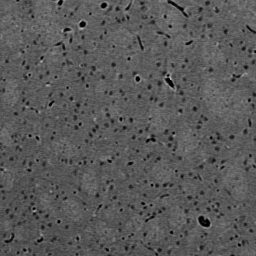
\includegraphics[width=\textwidth]{../figs/xray_sl84}
    \caption{Raw data\label{fig:xray}}
  \end{subfigure}
  \hspace{1em}
  \begin{subfigure}[b]{0.3\textwidth}
    \centering 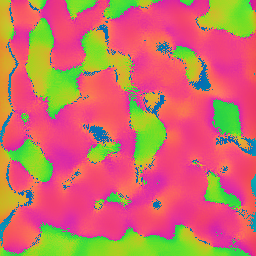
\includegraphics[width=\textwidth]{../figs/RGB_raw_d2_n7_sl84}
    \caption{Orientation estimate\label{fig:rgb_raw}}
  \end{subfigure}
  \hspace{1em}
  \begin{subfigure}[b]{0.30\textwidth}
    \centering 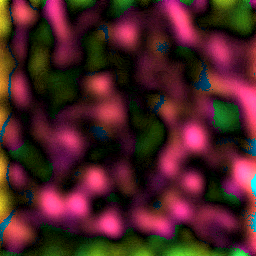
\includegraphics[width=\textwidth]{../figs/RGB_scaled_d2_n7_sl84}
    \caption{Intensity scaled by AI\label{fig:rgb_scaled}}
  \end{subfigure}
  \caption{(a)~Slice of a $256\times256\times256$ ROI in the raw xray data. The
    nominal voxel size is $1.2\times1.2\times1.2$ \textmu m$^3$. (b)~Orientation
    results. RGB color corresponds to column-row-slice (x, y, z) eigenvector
    components, respectively. (c)~Orientation results scaled by
    AI.\label{fig:sample}}
\end{figure}

\textbf{NOTE}: These results are different than those shown in group meeting
last week. I found an error in how I had implemented the partial derivative
filters, as well as how I was doing the AI scaling. The promising result from
these figures is that the structure tensor analysis seems to be successfully
identifying the axon bundles. Regions of high anisotropy (high intensity in
Figure~\ref{fig:rgb_scaled}) correspond to the axon bundles in
Figure~\ref{fig:xray}, and the orientations (color) within these regions are
relatively homogeneous.
  
A more rigorous sensitivity study is needed to validate the orientation
directions themselves. The fibers in Figure~\ref{fig:rgb_scaled} are
predominately red, indicating strong orientation in the $x$ direction.  To
verify, I made an orientation colormap in spherical coordinates, shown in
Figure~\ref{fig:cmap}. This colormap was created by mapping a 2D grid of polar
and azimuthal angles to 3D Cartesian coordinates, then scaling the $(x, y, z)$
results to 0--255 RGB values. I manually chose a few points within axon regions
of Figure~\ref{fig:rgb_raw} and found their spherical position using the actual
RGB values in Figure~\ref{fig:2Dcmap}.
\begin{figure}[h]
  \centering
  \begin{subfigure}[b]{0.48\textwidth}
    \centering 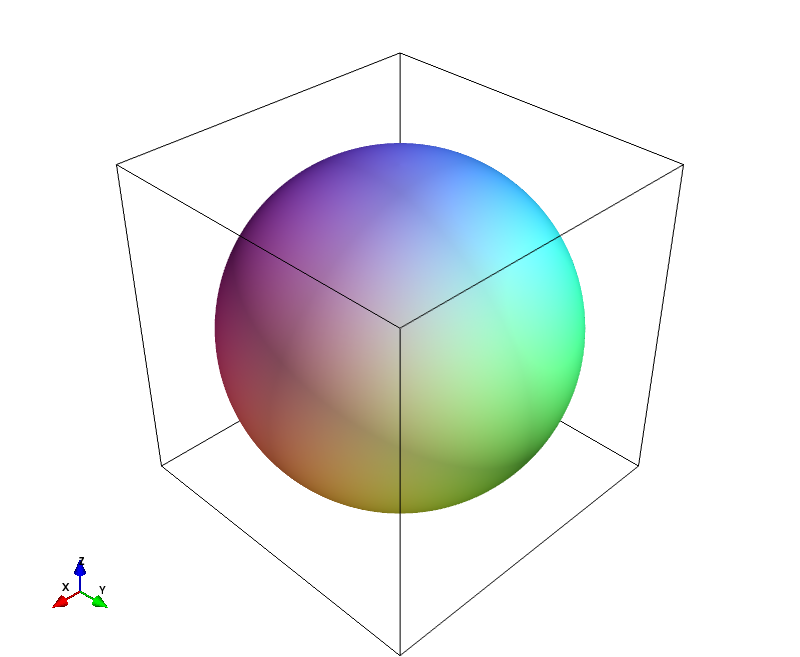
\includegraphics[width=\textwidth]{../figs/colormap_sphere}
    \caption{Spherical\label{fig:3Dcmap}}
  \end{subfigure}
  \begin{subfigure}[b]{0.48\textwidth}
    \centering 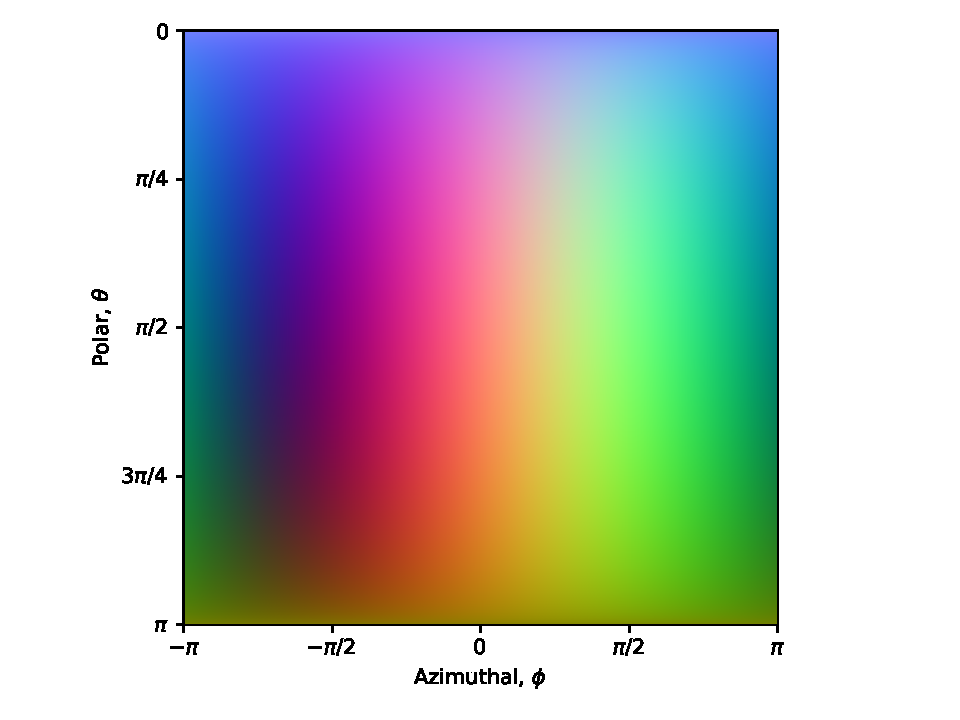
\includegraphics[width=\textwidth]{../figs/colormap}
    \caption{2D \label{fig:2Dcmap}}
  \end{subfigure}
  \caption{Orientation colormap. \label{fig:cmap}}
\end{figure}
This seemed to indicate that the current results are reporting the axons
traveling in the $xy$--plane ($\theta\approx\pi/2$), when (to my eye) they are
actually traveling more along the slice direction in the raw data, meaning that
there might be inconsistencies somewhere in how I have defined my coordinate
axes.
 
I have also experimented with visualizing the results as a 3D vector field.  The
pipeline is in progress, but I'm still working on the best way to threshold the
results; visualizing every vector in the volume looks extremely cluttered.

\subsection{Orientation Distribution Function}

Ultimately, we are interested in the distribution of orientations within an
ROI. As with the colormap above, we accomplish this by first reparameterizing
the orientations into spherical coordinates, with polar angle
$\theta \in [0,\pi]$ and azimuthal angle $\phi\in[-\pi,\pi]$:
\begin{align}
  \label{eq:sphcoords}
  r &= \sqrt{x^2 + y^2 + z^2}\\[5pt]
  \theta &= \text{cos}^{-1}\left(\frac{z}{r}\right)\\[5pt]
  \phi &= \text{tan}^{-1}\left(\frac{y}{x}\right)
\end{align}
A 2D histogram of $(\theta, \phi)$ orientations is generated with the
\href{https://docs.scipy.org/doc/numpy/reference/generated/numpy.histogram2d.html}{histogram2D}
function in the NumPy package, with bin locations determined by
\href{http://lgdv.cs.fau.de/uploads/publications/spherical_fibonacci_mapping_opt.pdf}{spherical
  Fibonacci sampling}, which produces approximately evenly spaced points on the
sphere. The histogram results are then visualized on a sphere with the
\href{http://docs.enthought.com/mayavi/mayavi/mlab.html}{mayavi} Python package,
with the radius of the sphere depending on the number of counts at that angular
location. Initial results are shown in Figure~\ref{fig:ODFs}.
\begin{figure}[h]
  \centering
  \begin{subfigure}[b]{0.48\textwidth}
    \centering 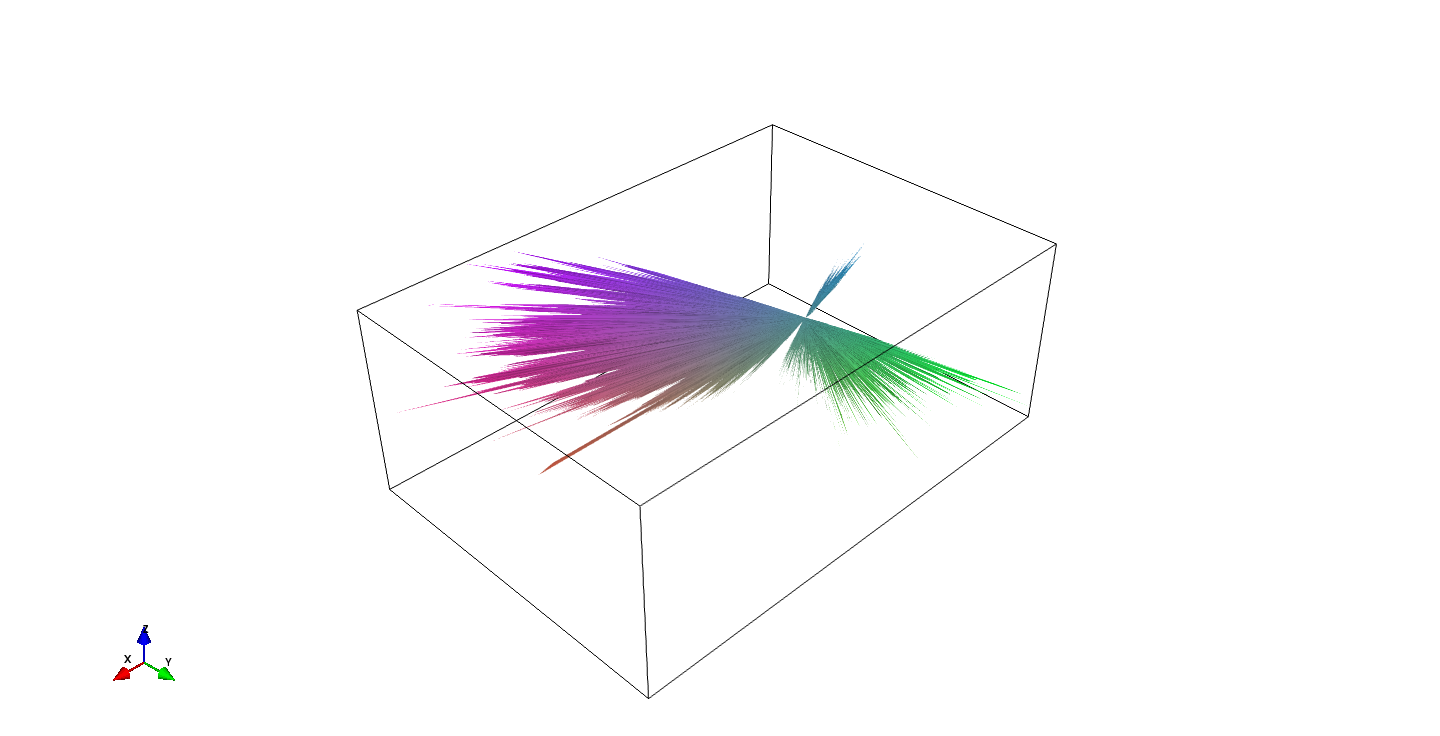
\includegraphics[width=\textwidth]{../figs/ODF_full_d2n7_view1}
    \caption{Raw ODF, view 1\label{fig:rawv1}}
  \end{subfigure}
  \hspace{1em}
  \begin{subfigure}[b]{0.48\textwidth}
    \centering 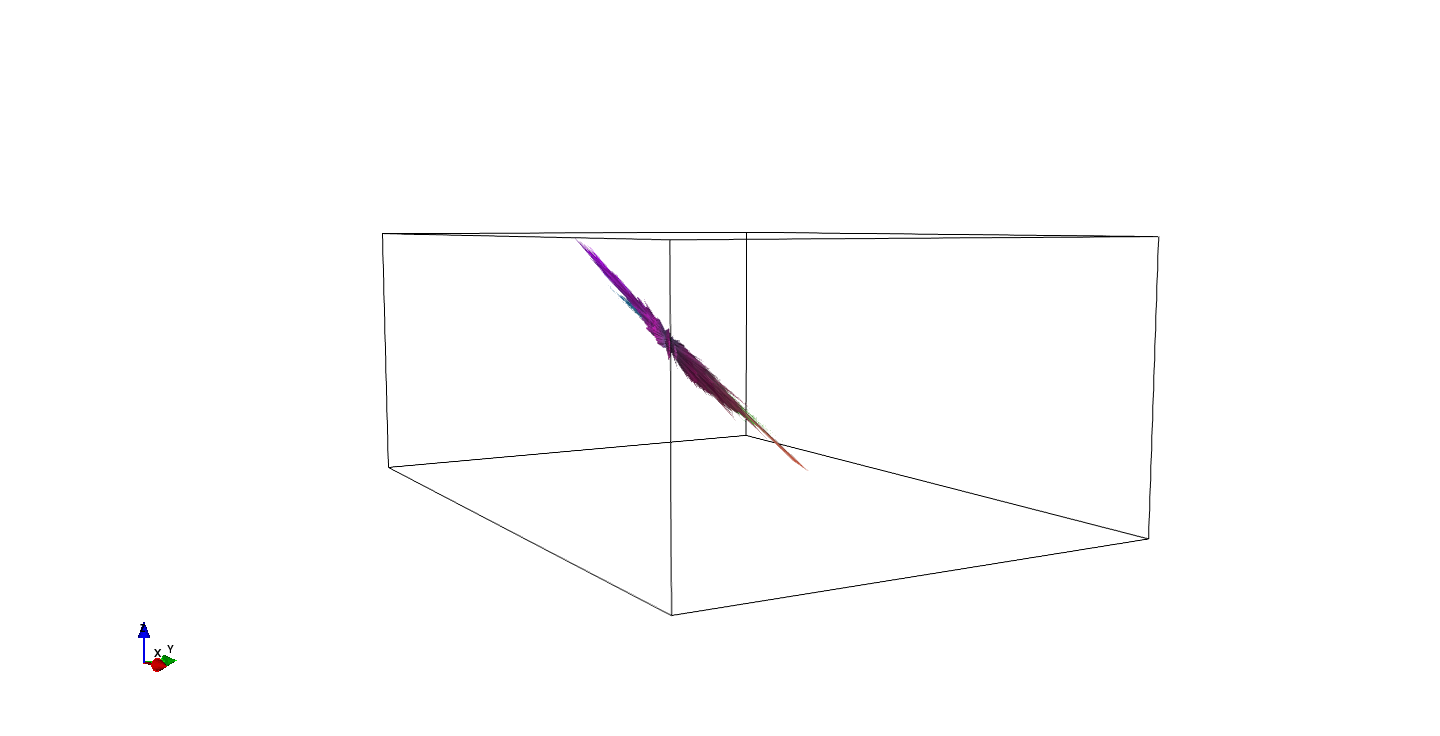
\includegraphics[width=\textwidth]{../figs/ODF_full_d2n7_view2}
    \caption{Raw ODF, view 2\label{fig:rawv2}}
  \end{subfigure}
  \vspace{2em}
  \begin{subfigure}[b]{0.48\textwidth}
    \centering 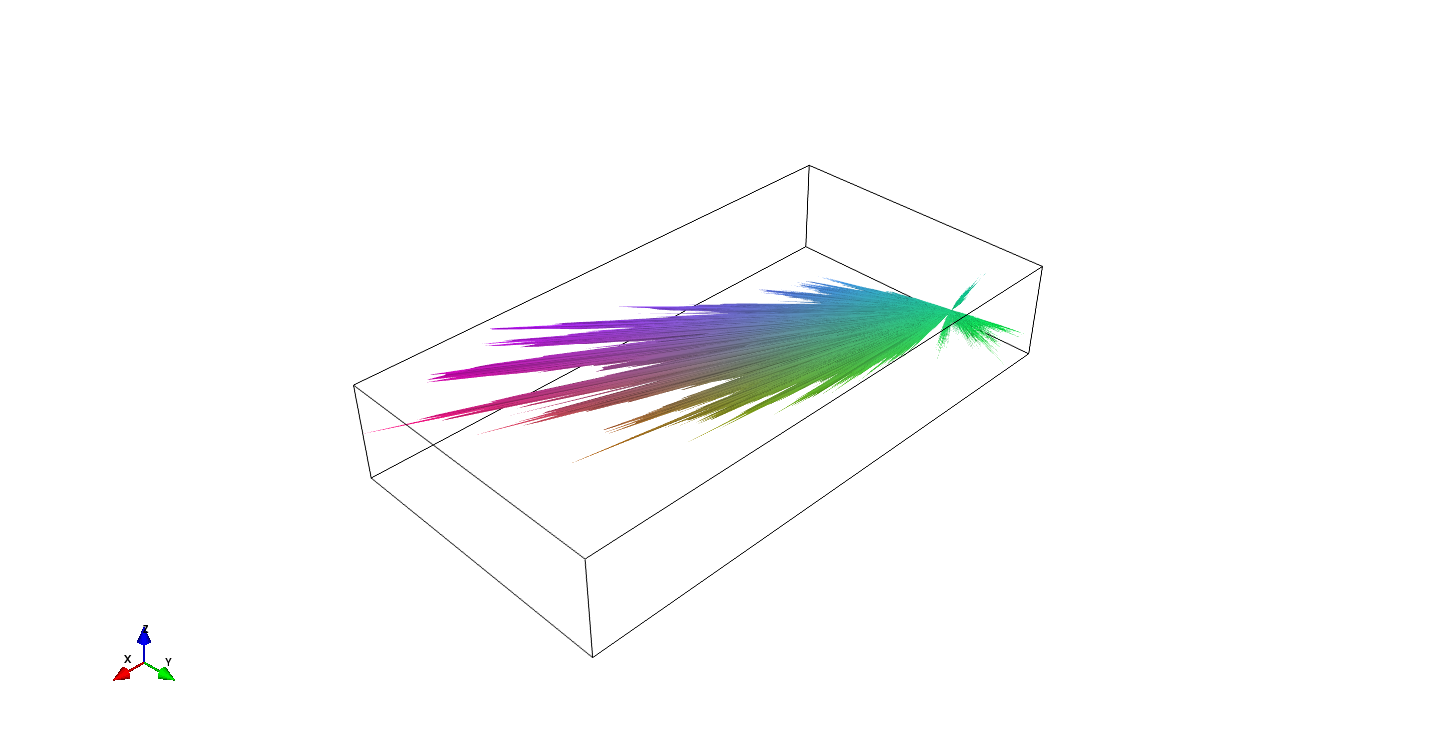
\includegraphics[width=\textwidth]{../figs/ODF_masked_d2n7_view1}
    \caption{AI-thresholded ODF, view 1\label{fig:maskedv1}}
  \end{subfigure}
  \hspace{1em}
  \begin{subfigure}[b]{0.48\textwidth}
    \centering 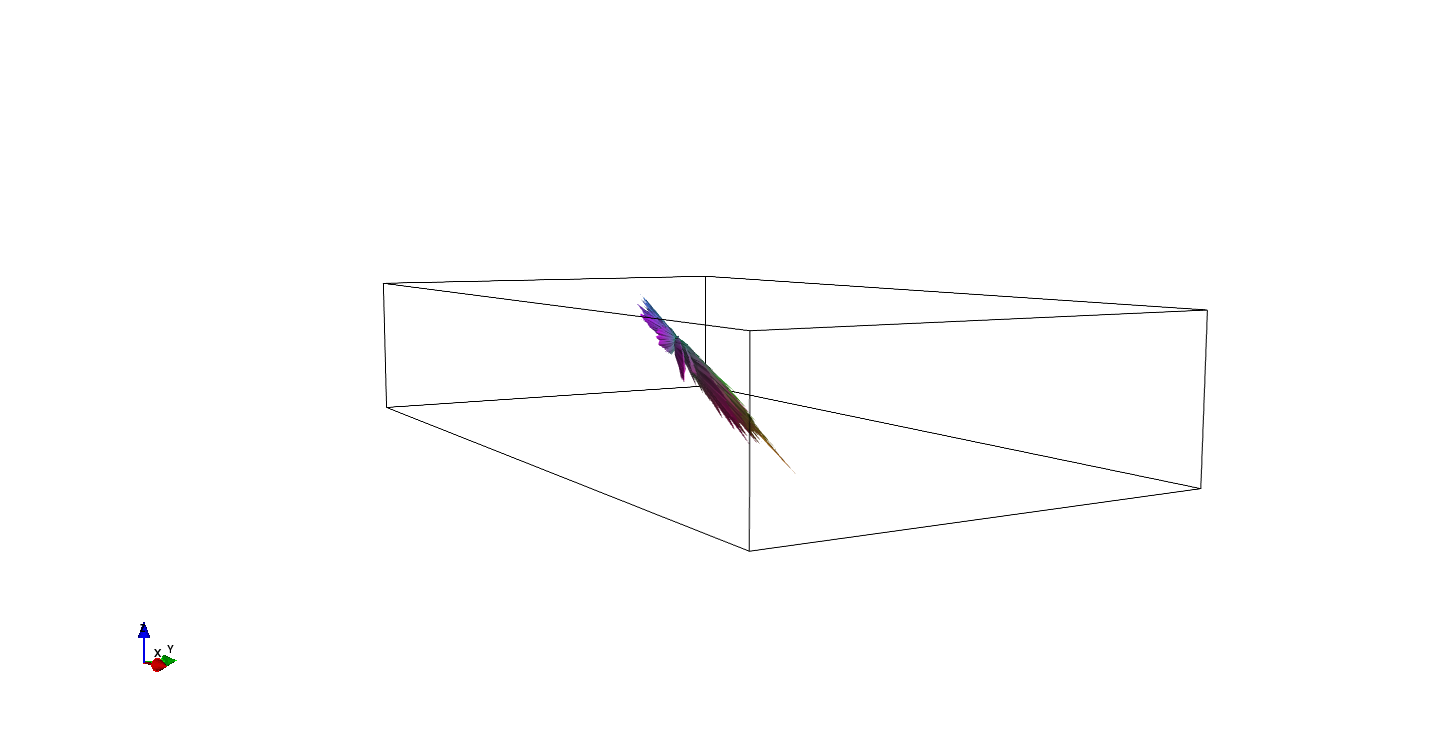
\includegraphics[width=\textwidth]{../figs/ODF_masked_d2n7_view2}
    \caption{AI-thresholded ODF, view 2\label{fig:maskedv2}}
  \end{subfigure}
  \caption{(a-b) Two views of the raw ODF, sampled with n=800 points on the
    sphere. (c-d) Two views of the same ODF, thresholded to only include voxels
    with AI~$>$ mean(AI). Note that the orientations fall narrowly into a single
    plane.\label{fig:ODFs}}
\end{figure}
Figures~\ref{fig:rawv1} and~\ref{fig:rawv2} depict the raw ODF for the entire
sample volume, while Figures~\ref{fig:maskedv1} and~\ref{fig:maskedv2} depict
the ODF after thresholding by AI~$>$ mean(AI). As expected, the AI thresholding
generates a more narrow, directed ODF. Also, as with the results in
Figure~\ref{fig:sample}, most orientations appear to fall more in line with the
positive $x$-axis than the $z$-axis, indicating an incorrect coordinate frame
definition at some point in the pipeline. It is also worth noting that most
orientations seem to be falling within a single plane, identified in
Figures~\ref{fig:rawv2} and ~\ref{fig:maskedv2}. Again, a rigorous sensitivity
study will allow us to validate the absolute orientations, as well as to
optimize the choice of AI metric and threshold value.

The next step is to expand this orientation distribution function on the
spherical harmonics for use in various comparison metrics with the MRI
distribution functions. We will also need to address how sensitive those results
are to $n$, the number of sampling points for the histogram.

  
\section{Current Issues / TODO list}
\begin{itemize}
\item Sensitivity study
  \begin{itemize}
  \item Segment myelinated axons from ROI and/or create fiber phantom
  \item Use segmented data / phantoms to validate coordinate frame
  \item Compare orientation/AI results from raw data to segmented fibers /
    phantom to optimize the choices of $\sigma_d$, $\sigma_n$, AI metric and AI
    threshold value
  \end{itemize}
\item Implement spherical harmonic expansion
  \begin{itemize}
  \item How sensitive is the expansion to the number of sampling bins?
  \end{itemize}
\item Gordon Conference
  \begin{itemize}
  \item Finish abstract
  \item Identify a few sample ROI in x-ray and MRI data for comparison.
  \item Potentially look at ROI registration for quantitative comparison
  \end{itemize}
\item Scalability
  \begin{itemize}
  \item With the current test parameters, it takes about 30 seconds on my
    Macbook to calculate the structure tensor results for this
    $256\times256\times100$, 6.6 Mb ROI
  \item I will do more detailed testing to find the bottlenecks. As we have
    discussed, I suspect I will need to look at implementing the convolutions in
    the Fourier domain.
  \end{itemize}
\end{itemize}



\bibliographystyle{ieeetr} \bibliography{structure-tensor-update}
\end{document}
